\chapter{Introduction}\label{introduction}

Social media has become an essential part of the modern life, enabling billions to share their stories, connect over shared interests, and participate in discussions on global events. These platforms function as virtual spaces where individuals form communities based on shared interests, values, or goals. Unlike physical communities, online communities allow for easier and more immediate grouping of individuals, as joining a community often requires minimal effort; simply clicking a button or following a page \citep{ellison:2007}. This ease of access fosters the creation of diverse and dynamic social ecosystems, where users interact under shared norms, behaviors, and communication styles unique to each community.

However, the aggregation of large numbers of individuals in online communities also increases the likelihood of negative behaviors, such as toxicity. Toxicity in online spaces refers to harmful actions, including hate speech, racism, sexism, and other forms of discrimination, often exacerbated by the anonymity and reduced social inhibitions that characterize digital environments \citep{suler:2005}. Such behaviors can disrupt community solidarity and harm individual users, making toxicity a significant challenge for social media platforms. To mitigate these issues, online communities establish rules and moderation systems to enforce acceptable behavior. Violations of these rules can result in penalties, such as bans or restrictions, depending on the platform's moderation policies.

This case study on Mastodon explores the dynamics of online communities, focusing on the challenges of toxicity and the role of moderation systems in digital spaces.

Just like every social media platform, Mastodon offers the posibility to interact with other people by publishing own posts, reacting on posts, or sharing posts. But Mastodon is a federated social media platform. Thereby federation means a special kind of decentralization. Traditional social media platforms as e.g. Twitter, Facebook or Instagram have a single central service all people use. Instead Mastodon has multiple services, so called instances, used by any number of people. These instances can communicate with each other and create a federated network. Users can freely choose an instance based on language, community rules, moderation policies, and topics of interest. Each instance is managed by its own administrators, who set and enforce local rules. \citep{mastodon:docs}

\begin{figure}[h]
    \centering
    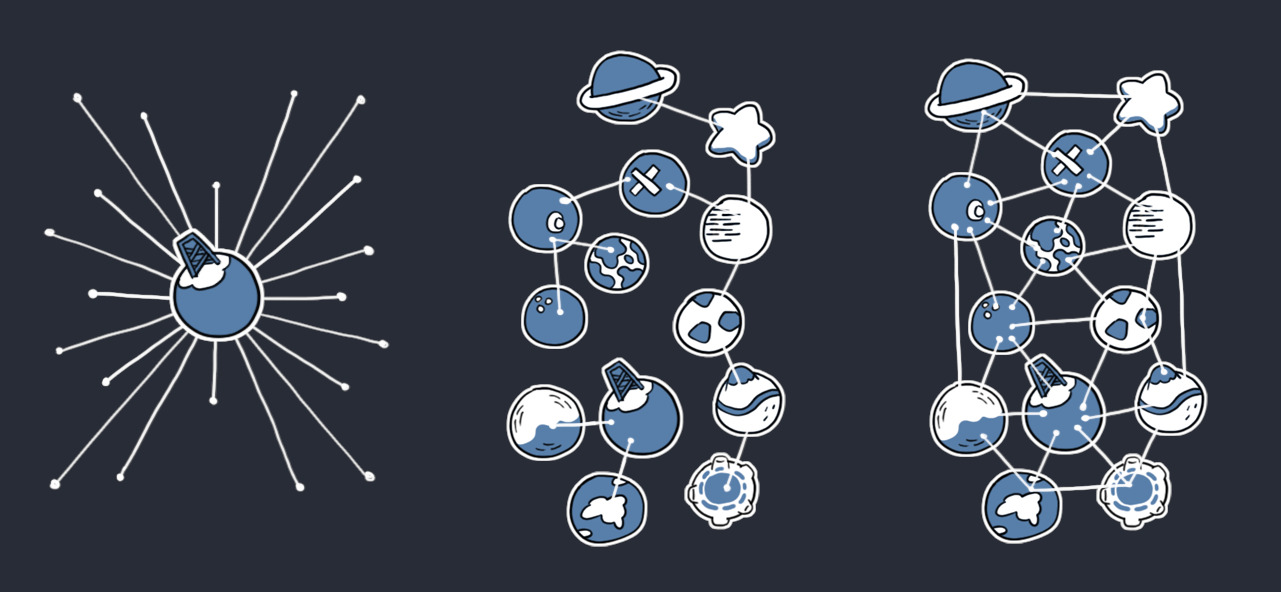
\includegraphics[width=\textwidth]{../material/network_models.jpg}
    \caption{From left to right: Centralized, Federated, Distributed, \citep{mastodon:docs}}
    \label{fig:network-models}
\end{figure}

To study the behaviour of online communities we use a dataset including 3.6 billion public mastodon posts from 1081 insances. The dataset was collected over 301 days from 2024 to 2025 \citep{ernst:2024}. By offering Metadata and the posted content, the dataset can be used to analyse the toxicity trends on the instances and the interaction between the instances.

\enlargethispage{\baselineskip}